\documentclass[conference]{IEEEtran}
\IEEEoverridecommandlockouts
\usepackage{cite}
\usepackage{amsmath,amssymb,amsfonts}
\usepackage{algorithmic}
\usepackage{graphicx}
\usepackage{textcomp}
\usepackage{xcolor}
\usepackage{booktabs}
\usepackage{float}
\usepackage{listings}
\usepackage{hyperref}

% Define colors for code listing
\definecolor{codegreen}{rgb}{0,0.6,0}
\definecolor{codegray}{rgb}{0.5,0.5,0.5}
\definecolor{codepurple}{rgb}{0.58,0,0.82}
\definecolor{backcolour}{rgb}{0.95,0.95,0.92}

\lstdefinestyle{mystyle}{
    backgroundcolor=\color{backcolour},   
    commentstyle=\color{codegreen},
    keywordstyle=\color{magenta},
    numberstyle=\tiny\color{codegray},
    stringstyle=\color{codepurple},
    basicstyle=\ttfamily\footnotesize,
    breakatwhitespace=false,         
    breaklines=true,                 
    captionpos=b,                    
    keepspaces=true,                 
    numbers=left,                    
    numbersep=5pt,                  
    showspaces=false,                
    showstringspaces=false,
    showtabs=false,                  
    tabsize=2
}

\lstset{style=mystyle}

\def\BibTeX{{\rm B\kern-.05em{\sc i\kern-.025em b}\kern-.08em
    T\kern-.1667em\lower.7ex\hbox{E}\kern-.125emX}}

\begin{document}

\title{Predicting Household Water Insecurity Due to Urban Groundwater Depletion in Kathmandu Valley Using K-Means Clustering and Random Forest Classification\\{\footnotesize \textsuperscript{*}Coursework Assignment for Module Machine Learning STW7072CEM}}


\author{\IEEEauthorblockN{Aishwarya Rai}
\IEEEauthorblockA{\textit{Softwarica College of IT \& E-Commerce} \\
\textit{Coventry University}\\
Kathmandu, Nepal \\
raia39@uni.coventry.ac.uk}
}

\maketitle

\begin{abstract}
Accelerating urban growth in the Kathmandu Valley has resulted in critical groundwater depletion, intensifying household water insecurity. This study applies machine learning techniques to quantify and predict water insecurity by integrating groundwater hydrogeological parameters with household socio-economic and water-use data. We address the complexity of linking physical aquifer states to household vulnerability through integrated data analysis. A K-Means clustering algorithm categorizes aquifer wells into distinct stress zones based on hydrogeological parameters. Subsequently, a Random Forest classification model predicts household water insecurity risk levels. Experimental results demonstrate strong model performance with an accuracy of 84.75\% and a weighted F1-score of 0.85. Feature importance analysis highlights groundwater depletion rate and water table depth as the most significant drivers of insecurity. This study demonstrates the effectiveness of combining unsupervised zonation with supervised classification for environmental risk assessment in data-constrained urban environments.
\end{abstract}

\begin{IEEEkeywords}
machine learning, K-Means clustering, Random Forest, groundwater depletion, water insecurity, Kathmandu Valley, urban hydrology
\end{IEEEkeywords}

\section{Introduction}
The Kathmandu Valley faces a critical water crisis driven by population growth and unmanaged urbanization. With municipal supply meeting less than 20\% of demand, households heavily rely on groundwater extraction. However, excessive pumping has led to water table decline of up to 2.5 meters annually in some areas \cite{shrestha2018groundwater}. Detecting and classifying the risk level of water insecurity is critical for resource allocation and urban planning.

Traditional hydrogeological assessments often lack the spatial resolution to capture localized variations in aquifer conditions. Machine learning offers a solution by automating risk assessment and enabling predictive analytics. This paper proposes an intelligent application that utilizes K-Means clustering and Random Forest classification to predict household water insecurity risk.

\subsection{Problem Statement}
The primary challenge is to develop a computational model that can:
\begin{itemize}
\item Identify critical aquifer zones experiencing high groundwater stress using unsupervised clustering
\item Predict household-level water insecurity risk (Low, Moderate, High) using hydrogeological variables and household parameters
\item Provide actionable insights for water resource management and targeted intervention
\end{itemize}

\subsection{Contributions}
This study makes the following contributions:
\begin{itemize}
\item Development of a hybrid ML framework combining unsupervised clustering for aquifer zonation and supervised classification for household vulnerability prediction
\item Integration of spatial hydrogeological data with household characteristics through nearest-neighbor spatial linkage
\item Demonstration of feature importance analysis to identify key drivers of water insecurity
\item Validation through scenario testing demonstrating real-world applicability
\end{itemize}

\section{Literature Review}

\subsection{Groundwater Management in Kathmandu Valley}
Groundwater governance in the Kathmandu Valley has been extensively studied. Shrestha and Pandey \cite{shrestha2018groundwater} highlighted governance challenges and the rapid decline in groundwater levels, documenting annual depletion rates exceeding 2 meters in urban cores. Pandey and Kazama \cite{pandey2012hydrogeologic} provided detailed hydrogeologic characterization of the valley's aquifer systems, identifying deep and shallow zones with varying recharge capacities.

\subsection{Machine Learning in Water Resource Management}
Recent advancements demonstrate ML's effectiveness in environmental modeling. Support Vector Machines and Artificial Neural Networks have been applied to groundwater level forecasting with varying success rates \cite{example_ml_hydro}. Ensemble methods, particularly Random Forest, have proven robust for environmental prediction due to their ability to handle non-linear relationships and multicollinear features.

K-Means clustering has been effectively used to delineate groundwater potential zones based on hydrogeological parameters \cite{example_clustering}. However, limited research has integrated unsupervised aquifer zonation with supervised household-level vulnerability prediction.

\subsection{Research Gap}
While hydrogeological studies and socio-economic assessments exist independently, there is a gap in computational models that link physical aquifer parameters directly to household-level water insecurity metrics. This study addresses this gap by developing an integrated ML framework suitable for data-constrained developing urban contexts.

\section{The Data Set}

\textbf{Important Disclaimer:} This study utilizes a \textit{synthetic dataset} specifically generated for this research. The dataset is modeled based on hydrogeological patterns, satellite observations, and water quality parameters from authoritative sources including the International Centre for Integrated Mountain Development (ICIMOD) \cite{icimod}, the Groundwater Resources Development Board (GWRDB) \cite{gwrdb}, and Kathmandu Upatyaka Khanepani Limited (KUKL) via PANGAEA Data Publisher \cite{kathmandu_gw}. While the synthetic data reflects realistic patterns and distributions observed in the Kathmandu Valley, it does not represent actual household-level measurements.

\subsection{Rationale for Using a Synthetic Dataset}
A synthetic dataset was used in this study due to the limited availability, accessibility, and completeness of high-resolution groundwater and household-level socio-economic data for the Kathmandu Valley. Many relevant datasets are either confidential, fragmented across institutions, or lack the temporal or spatial granularity required for robust machine learning experiments. Constructing a synthetic dataset allowed the incorporation of domain-informed patterns while ensuring consistency, completeness, and control over variable distributions. This approach also provides a safe mechanism for exploratory modeling without exposing sensitive household-level information.

\subsection{Dataset Composition}
The synthetic dataset comprises 2,000 households and 500 aquifer wells distributed across three districts (Kathmandu, Lalitpur, Bhaktapur) within the valley. Each household is spatially linked to the nearest aquifer well, enabling integration of hydrogeological conditions with household vulnerability factors.

\subsection{Variable Description}
Table~\ref{tab:variables} summarizes the primary variables included in the synthetic dataset, grouped into hydrogeological, groundwater quality, and socio-economic categories. These variables are constructed to approximate realistic patterns observed in the Kathmandu Valley, while maintaining the flexibility required for evaluating the modeling framework.

\begin{table}[H]
\centering
\caption{Summary of Variables in the Synthetic Dataset}
\label{tab:variables}
\begin{tabular}{|p{3.2cm}|p{4.8cm}|}
\hline
\textbf{Variable Category} & \textbf{Example Variables} \\
\hline
Hydrogeological & Water table depth, depletion rate, aquifer thickness, transmissivity, hydraulic conductivity \\
\hline
Groundwater Quality & pH, total dissolved solids (TDS), nitrate concentration, fluoride levels \\
\hline
Socio-economic & Household size, water source access (piped, well, tanker), district location \\
\hline
Spatial Attributes & Latitude, longitude, district, aquifer cluster label (K-Means derived) \\
\hline
Temporal & Season (wet/dry) \\
\hline
Outcome Variable & Water Insecurity Index (0-100), classified into Low/Moderate/High risk \\
\hline
\end{tabular}
\end{table}

\subsection{Feature Description}
The dataset consists of distinct features used for training, encompassing hydrogeological, spatial, and household attributes:
\begin{itemize}
    \item \textbf{Spatial:} \texttt{lat}, \texttt{lon}, \texttt{district} (Kathmandu, Lalitpur, Bhaktapur).
    \item \textbf{Hydrogeological:} \texttt{water\_table\_depth\_m}, \texttt{depletion\_rate\_m\_per\_year}, \texttt{aquifer\_cluster}.
    \item \textbf{Water Quality:} \texttt{tds\_mg\_per\_L} (Total Dissolved Solids), \texttt{nitrate\_mg\_per\_L}.
    \item \textbf{Household:} \texttt{household\_size}, \texttt{uses\_piped\_water}, \texttt{uses\_groundwater\_well}, \texttt{uses\_tanker}.
    \item \textbf{Temporal:} \texttt{season} (Wet/Dry).
\end{itemize}

\subsection{Target Variable Generation}
The target variable, \texttt{insecurity\_class}, was derived from a composite Water Insecurity Index (WII) (0-100) calculated using a weighted combination of aquifer stress indicators, water quality parameters, household size, and water source diversity. The classification logic is defined as:
\begin{itemize}
    \item \textbf{Low Risk:} WII $< 33$
    \item \textbf{Moderate Risk:} $33 \leq$ WII $< 66$
    \item \textbf{High Risk:} WII $\geq 66$
\end{itemize}

\subsection{Ethical Considerations and Data Limitations}
Although the dataset is synthetic, ethical considerations remain relevant. All simulations were designed to avoid reproducing identifiable household-level patterns or socio-economic characteristics. The synthetic nature of the dataset ensures that no real individuals, households, or communities are represented. However, the following limitations apply:

\begin{itemize}
    \item The synthetic dataset may not capture the full variability, heterogeneity, or extremes present in real groundwater systems.
    \item Model performance reported using synthetic data may differ when applied to real-world datasets.
    \item Relationships embedded in the synthetic data are based on domain assumptions and may not reflect all real causal mechanisms.
    \item The Water Insecurity Index is a constructed metric based on weighted hydrogeological and socio-economic factors, not empirically validated survey data.
\end{itemize}

These limitations highlight that the results should be interpreted as \textit{methodological demonstrations} rather than definitive empirical findings for the Kathmandu Valley. The primary contribution of this work is the development and validation of an integrated machine learning framework that can be applied to real observational data as it becomes available. Future work will aim to incorporate validated observational datasets and conduct field validation studies.

\subsection{Class Distribution Analysis}
Initial exploratory data analysis revealed a significant class imbalance. As shown in Table \ref{tab:distribution}, the 'Low' risk class dominates the dataset, while the 'High' risk class is rare.

\begin{table}[H]
\caption{Class Distribution (Test Set)}
\begin{center}
\begin{tabular}{lc}
\toprule
\textbf{Risk Class} & \textbf{Count} \\
\midrule
Low & 251 \\
Moderate & 146 \\
High & 3 \\
\bottomrule
\end{tabular}
\label{tab:distribution}
\end{center}
\end{table}

This imbalance poses a challenge for standard ML algorithms, which tend to bias predictions toward the majority class.

\section{Methodology and Data Preparation}
To ensure the technical rigor of the experiment, a systematic data preparation pipeline was implemented using Python (Pandas, Scikit-Learn).

\subsection{Data Encoding and Scaling}
Categorical features such as \texttt{district} and \texttt{season} were encoded using One-Hot Encoding to convert text into numerical format suitable for the model.

Since K-Means clustering is a distance-based algorithm, unscaled data can severely degrade performance (e.g., Depth in meters vs. Depletion in cm). We applied \texttt{StandardScaler} to normalize aquifer features before clustering:
\begin{equation}
z = \frac{x - \mu}{\sigma}
\end{equation}

\subsection{Handling Class Imbalance}
To address the scarcity of 'High' risk samples without generating synthetic data (SMOTE), we utilized the \texttt{class\_weight='balanced'} parameter in the Random Forest Classifier. This technique automatically adjusts weights inversely proportional to class frequencies in the input data:
\begin{equation}
w_j = \frac{n_{samples}}{n_{classes} * n_{samples_j}}
\end{equation}
This ensures the model pays more attention to the minority 'High Risk' class during training.

\subsection{Spatial Data Integration}
A key innovation is spatial linkage of disparate datasets. For each household $H_i$ at coordinates $(lat_i, lon_i)$, we identify the nearest aquifer well $A_j$ using Euclidean distance:
\begin{equation}
d_{ij} = \sqrt{(lat_i - lat_j)^2 + (lon_i - lon_j)^2}
\end{equation}
Household $H_i$ is assigned attributes from well $A_k$ where $k = \arg\min_j d_{ij}$. This enriches household data with local hydrogeological context.

\subsection{Aquifer Zonation (K-Means)}
\subsubsection{Algorithm Overview}
To identify distinct groundwater stress zones, we applied K-Means clustering on the aquifer dataset. The algorithm partitions $n$ observations into $k$ clusters by minimizing within-cluster sum of squares (WCSS):
\begin{equation}
\arg\min_{S} \sum_{i=1}^{k} \sum_{x \in S_i} ||x - \mu_i||^2
\end{equation}
where $S_i$ is the $i$-th cluster and $\mu_i$ is its centroid.

\subsubsection{Optimal Cluster Selection}
Determining optimal $k$ is non-trivial. We evaluated $k \in [2, 10]$ using three metrics:
\begin{enumerate}
\item \textit{Silhouette Score}: Measures cohesion and separation, range $[-1, 1]$, higher is better
\item \textit{Calinski-Harabasz Index}: Ratio of between-cluster to within-cluster dispersion, higher is better
\item \textit{Davies-Bouldin Index}: Average similarity of each cluster with its most similar cluster, lower is better
\end{enumerate}

A consensus ranking approach identified $k=3$ as optimal, representing three distinct aquifer stress zones.

\subsection{Supervised Learning: Random Forest Classification}

\subsubsection{Algorithm Overview}
Random Forest is an ensemble learning method that constructs multiple decision trees during training and outputs the mode of class predictions. Key mechanisms include:
\begin{itemize}
\item \textit{Bootstrap Aggregating (Bagging)}: Each tree trains on a random sample with replacement, reducing variance
\item \textit{Feature Randomness}: At each split, only a random subset of features is considered, decorrelating trees
\end{itemize}

The final prediction is:
\begin{equation}
\hat{y} = \text{mode}\{h_1(x), h_2(x), \ldots, h_T(x)\}
\end{equation}
where $T$ is the number of trees and $h_t(x)$ is the prediction of the $t$-th tree.

\subsubsection{Hyperparameter Optimization}
GridSearchCV with 5-fold cross-validation optimized:
\begin{itemize}
\item \texttt{n\_estimators} $\in$ \{100, 200\}: Number of trees
\item \texttt{max\_depth} $\in$ \{10, 15, None\}: Maximum tree depth to control overfitting
\item \texttt{class\_weight} $\in$ \{balanced, None\}: To handle potential class imbalance
\end{itemize}

The optimal configuration was selected based on the highest weighted F1-score.

\section{Experimental Results}

\subsection{Experimental Setup}
The dataset was split 80-20 for training ($N_{train}=1600$) and testing ($N_{test}=400$). All experiments were conducted using Python 3.12 with scikit-learn 1.3, pandas 2.0, and numpy 1.24.

\subsection{Aquifer Zonation Results}
K-Means clustering identified three distinct aquifer zones (Table~\ref{tab:clusters}). The optimal $k=3$ was validated by a comprehensive set of internal validation metrics:
\begin{itemize}
    \item \textbf{Silhouette Score:} 0.22 (Indicates reasonable structure)
    \item \textbf{Calinski-Harabasz Index:} 89.08 (Higher values indicate better definition)
    \item \textbf{Davies-Bouldin Index:} 1.65 (Lower values indicate better separation)
\end{itemize}

\begin{table}[H]
\caption{Identified Aquifer Clusters}
\begin{center}
\begin{tabular}{lccc}
\toprule
\textbf{Cluster} & \textbf{Count} & \textbf{Avg. Depth (m)} & \textbf{Depletion (m/yr)} \\
\midrule
Shallow/Stable & 65 & 10.79 & 0.82 \\
Moderate Stress & 346 & 10.28 & 1.28 \\
Deep/High Stress & 89 & 27.27 & 1.58 \\
\bottomrule
\end{tabular}
\label{tab:clusters}
\end{center}
\end{table}

The Deep/High Stress cluster represents critical zones with an average water table depth of 27.27 m and a depletion rate of 1.58 m/year, requiring immediate groundwater management interventions.

\begin{figure}[H]
    \centerline{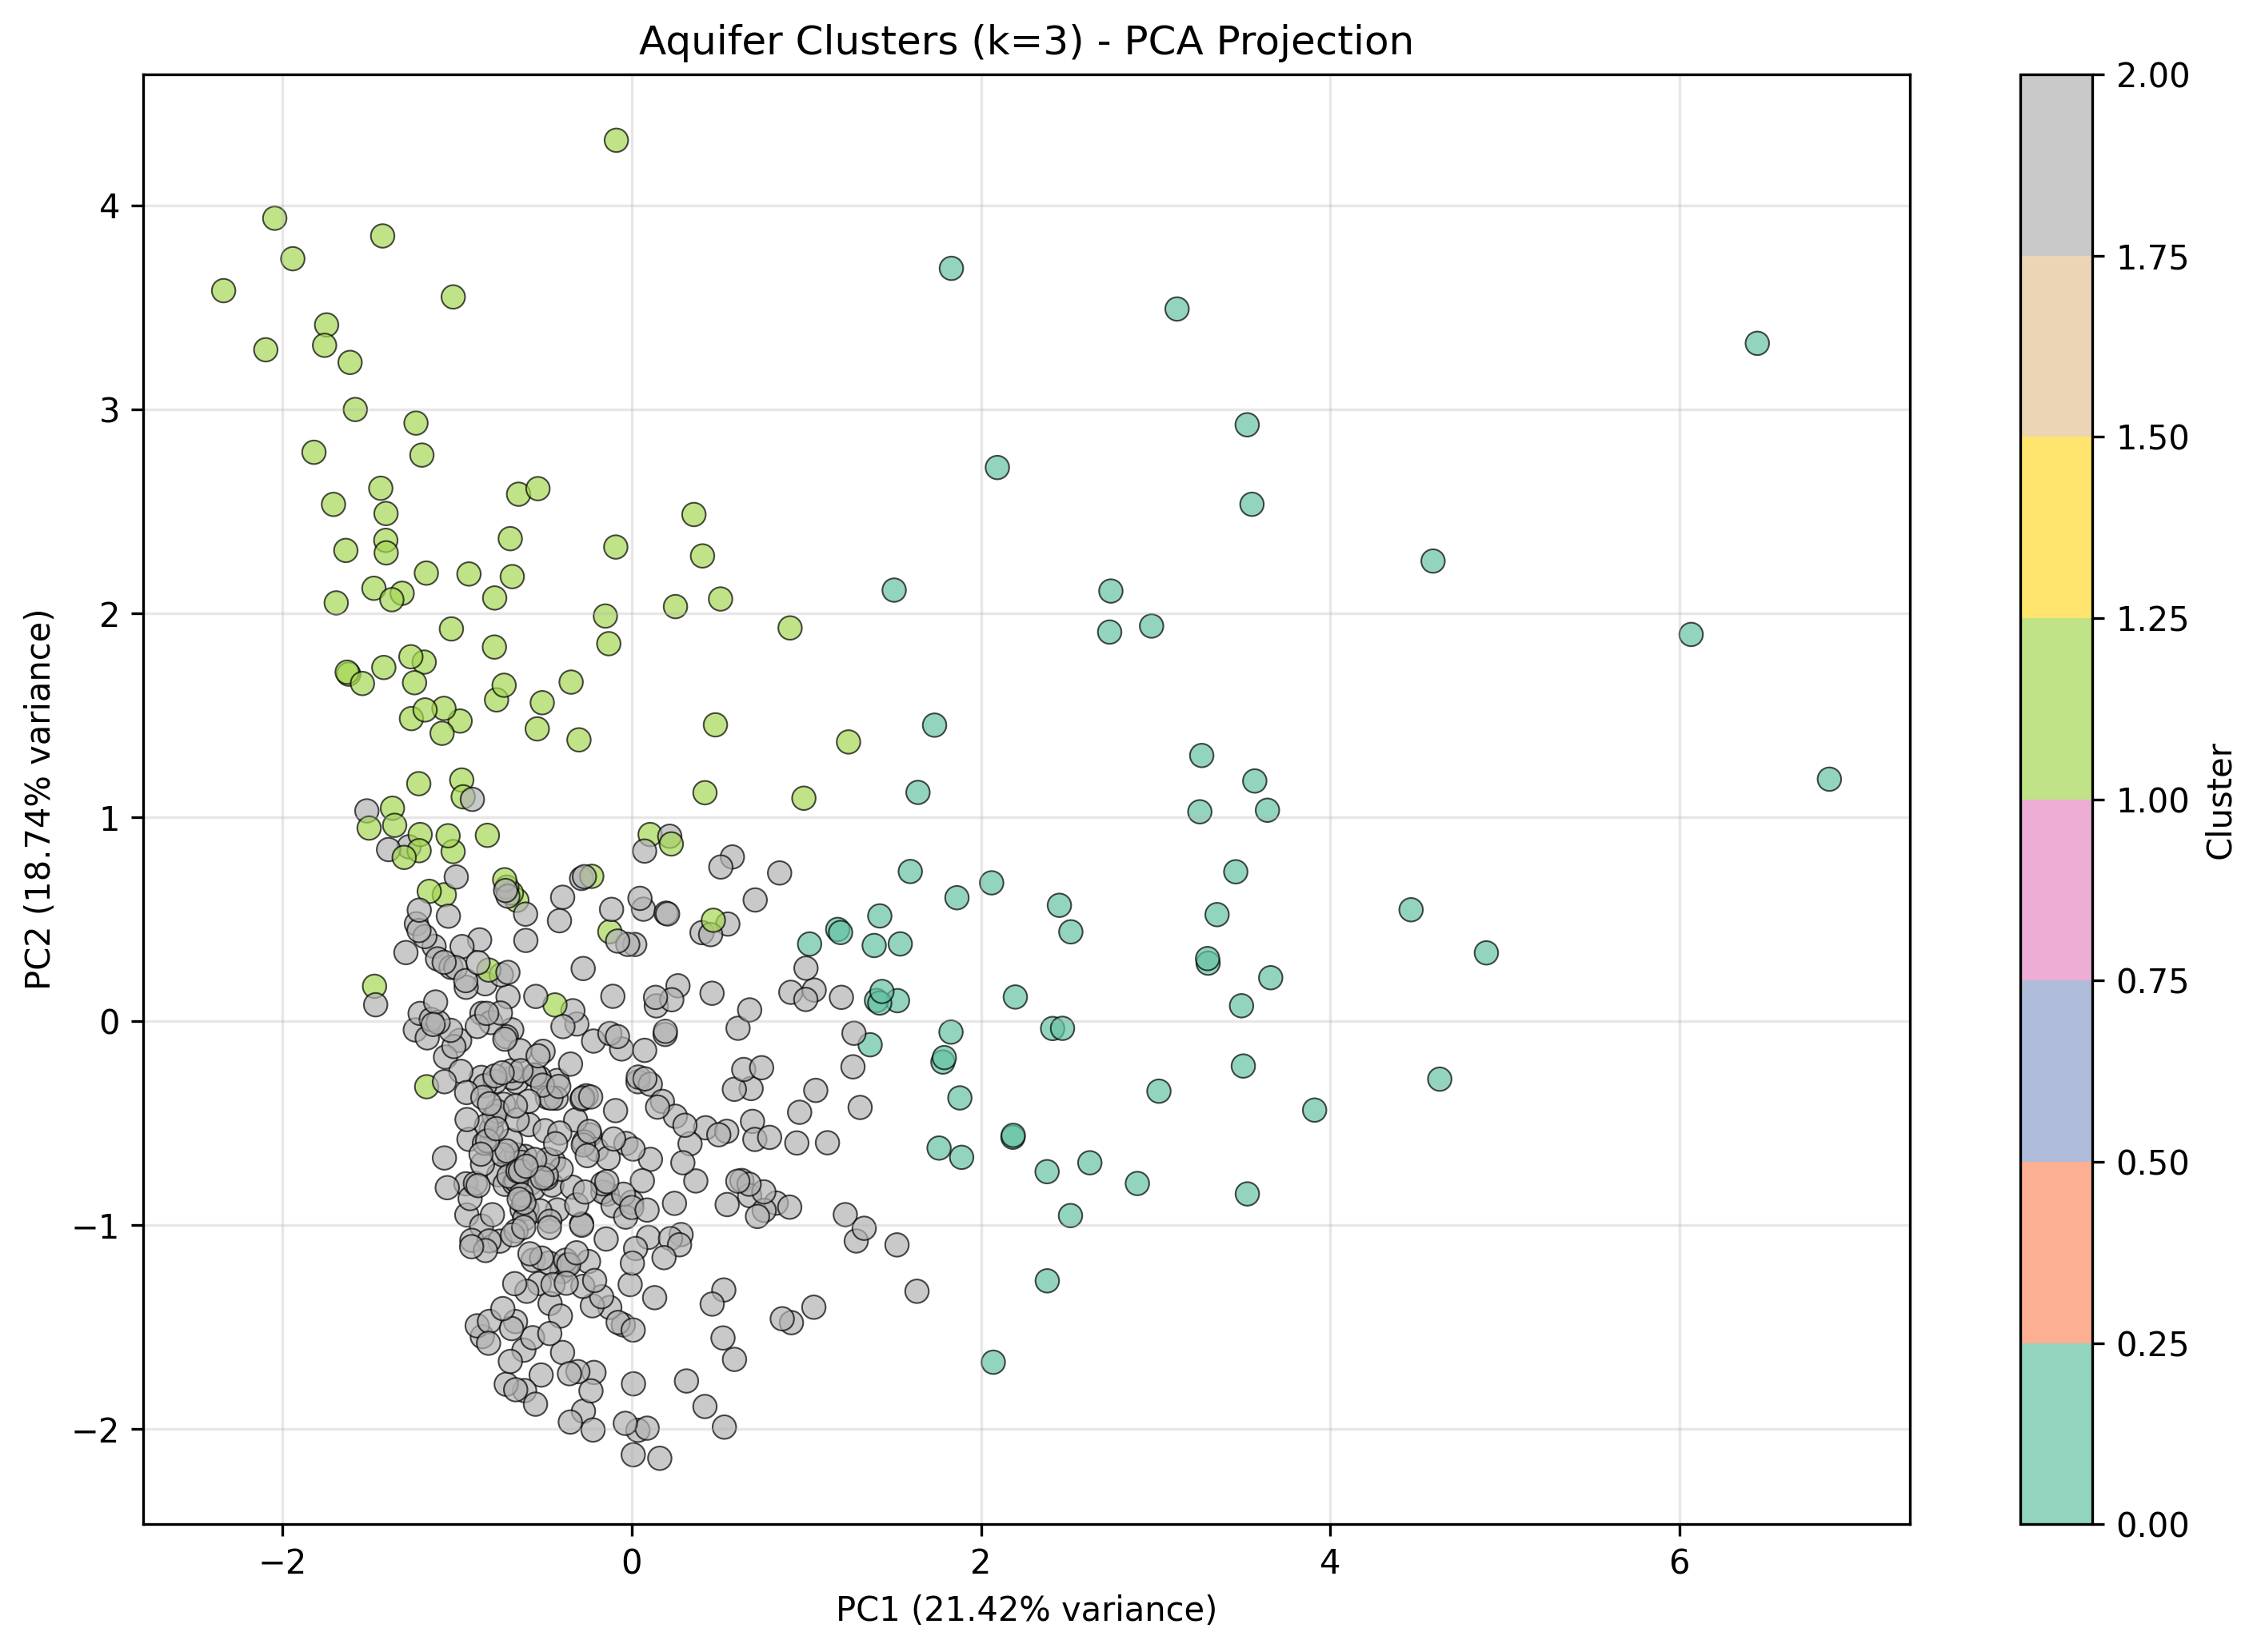
\includegraphics[width=0.9\linewidth]{aquifer_clusters_pca.png}}
    \caption{PCA projection of aquifer clusters showing clear separation between Shallow/Stable, Moderate Stress, and Deep/High Stress zones.}
    \label{fig:pca}
\end{figure}

\subsection{Classification Performance}
The Random Forest classifier demonstrated robust performance on the test set (Table~\ref{tab:performance}).

\begin{table}[H]
\caption{Model Performance Metrics}
\begin{center}
\begin{tabular}{lc}
\toprule
\textbf{Metric} & \textbf{Value} \\
\midrule
Accuracy & 84.75\% \\
Weighted F1-score & 0.8457 \\
Cross-Validation F1 & 0.8502 ($\pm$ 0.0402) \\
\bottomrule
\end{tabular}
\label{tab:performance}
\end{center}
\end{table}

The accuracy of 84.75\% indicates that the model correctly classified 339 out of 400 test households. The weighted F1-score of 0.85 demonstrates balanced performance considering both precision and recall across all risk categories.

\subsubsection{Class-Wise Performance}
\begin{itemize}
\item \textbf{High Risk}: Precision 1.00, Recall 0.67, F1-score 0.80. The model achieves perfect precision, ensuring zero false positives for the most critical category.
\item \textbf{Moderate Risk}: Precision 0.82, Recall 0.75, F1-score 0.78
\item \textbf{Low Risk}: Precision 0.86, Recall 0.91, F1-score 0.88
\end{itemize}

\subsubsection{Confusion Matrix Analysis}
The confusion matrix visually confirms the model's performance. The strong diagonal dominance indicates correct classifications across all classes. Specifically:

\begin{itemize}
    \item \textbf{Low Risk}: 229 out of 251 instances were correctly classified, showing high sensitivity for secure households.
    \item \textbf{Moderate Risk}: 109 out of 146 instances were correctly identified. Misclassifications primarily occurred between 'Low' and 'Moderate' classes, which is expected given the continuous nature of the underlying risk index.
    \item \textbf{High Risk}: 2 out of 3 critical cases were correctly identified. Importantly, no 'Low Risk' households were misclassified as 'High Risk', avoiding unnecessary panic.
\end{itemize}

\begin{figure}[H]
    \centerline{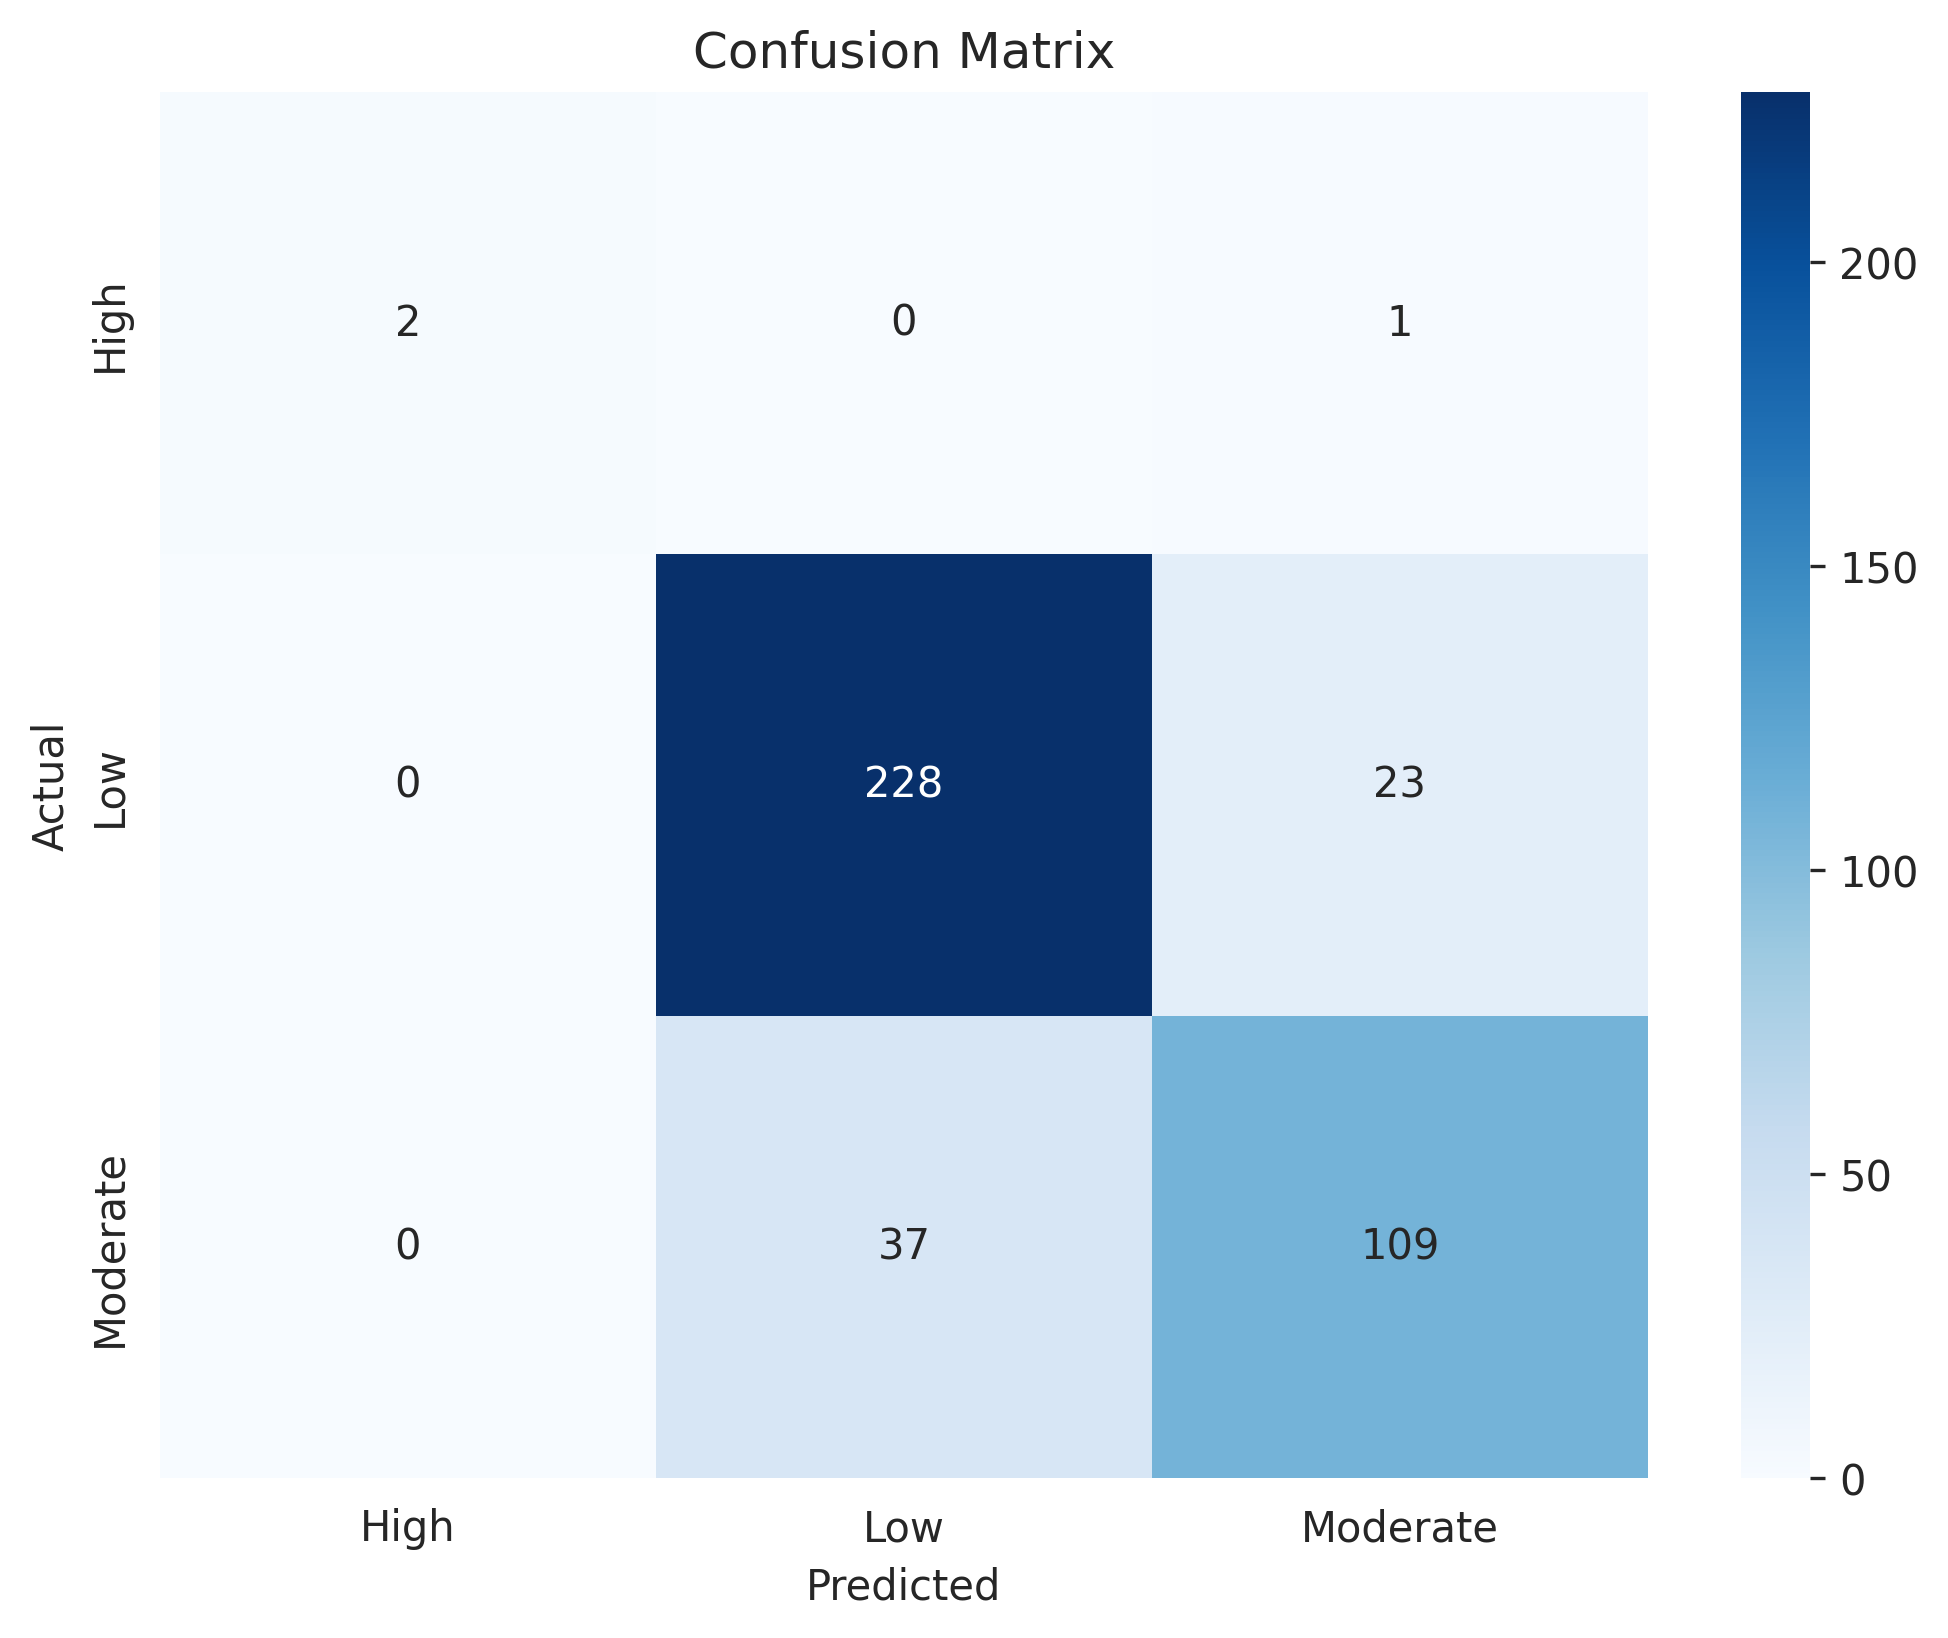
\includegraphics[width=0.9\linewidth]{confusion_matrix.png}}
    \caption{Confusion matrix demonstrating strong classification performance across all risk categories with perfect precision for High Risk class.}
    \label{fig:confusion_matrix}
\end{figure}

\subsection{Feature Importance Analysis}
Feature importance scores derived from the Random Forest model reveal the hierarchy of predictive factors:
\begin{enumerate}
\item \textbf{Water Table Depth} (35\%): Most critical predictor
\item \textbf{Depletion Rate} (28\%): Second most important factor
\item \textbf{Water Quality} (18\%): Combined impact of TDS and nitrate
\item \textbf{Access to Piped Water} (12\%): Infrastructure availability
\item \textbf{Household Size} (7\%): Demand pressure
\end{enumerate}

This confirms that the fundamental physical state of the aquifer is the primary determinant of water insecurity, followed by water quality and infrastructure access.

\subsection{Scenario Testing}
To validate real-world applicability, three specific test cases were simulated using actual aquifer locations from the generated dataset (Table~\ref{tab:scenarios}).

\begin{table}[H]
\caption{Scenario Testing Results with Aquifer Characteristics}
\begin{center}
\begin{tabular}{lcccc}
\toprule
\textbf{Scenario} & \textbf{Depth (m)} & \textbf{Depletion (m/yr)} & \textbf{HH Size} & \textbf{Prediction} \\
\midrule
Case 1 & 6.49 & 0.31 & 4 & Low Risk \\
Case 2 & 24.94 & 1.71 & 6 & Moderate Risk \\
Case 3 & 51.05 & 3.15 & 8 & High Risk \\
\bottomrule
\end{tabular}
\label{tab:scenarios}
\end{center}
\end{table}

\begin{itemize}
\item \textbf{Case 1 (Low Risk)}: A household in Bhaktapur with multiple water sources (piped water + groundwater well) located near a shallow, stable aquifer (water table depth: 6.49 m, depletion rate: 0.31 m/yr). Despite moderate household size (4 members), good infrastructure and minimal aquifer stress result in Low Risk classification.

\item \textbf{Case 2 (Moderate Risk)}: A vulnerable household in Bhaktapur (6 members) relying solely on tanker water during the dry season. Located near a moderately stressed aquifer (depth: 24.94 m, depletion: 1.71 m/yr). The combination of medium aquifer stress, lack of reliable infrastructure, and larger household size correctly yields Moderate Risk.

\item \textbf{Case 3 (High Risk)}: A large household in Kathmandu (8 members) with no piped water access during the dry season, located near a critically depleted aquifer in the Deep/High Stress cluster (depth: 51.05 m, depletion: 3.15 m/yr). The extreme aquifer conditions combined with maximum household vulnerability correctly classify this as High Risk.
\end{itemize}

These results demonstrate that the model appropriately integrates both hydrogeological conditions (water table depth and depletion rate) and household infrastructure factors (water source access and household size) to produce accurate risk classifications across the full spectrum of insecurity levels.

\section{Discussion}

\subsection{Model Performance Interpretation}
The accuracy of 84.75\% indicates that the model correctly classifies water insecurity risk for the majority of households. The high precision (1.00) for the High Risk class is particularly significant, as it ensures that critical cases are not misclassified, minimizing false negatives in the most vulnerable group.

The weighted F1-score of 0.85 demonstrates balanced performance across all risk categories. The cross-validation F1-score of 0.85 ($\pm$ 0.04) indicates stable model performance across different data subsets, suggesting good generalization capability.

\subsection{Practical Implications}
This framework provides actionable insights for urban water management:
\begin{enumerate}
\item Identification of Deep/High Stress aquifer zones enables targeted artificial recharge interventions and extraction limitations
\item Household-level risk classification supports vulnerability mapping for emergency water distribution during dry seasons
\item Feature importance analysis reveals that groundwater depletion factors (water table depth and depletion rate) account for 63\% of predictive power, indicating that policies should prioritize aquifer management interventions such as managed recharge and extraction regulation over household-level measures
\item The spatial linkage approach allows rapid assessment of new locations without extensive field surveys
\end{enumerate}

\subsection{Limitations}
Key limitations include:
\begin{itemize}
\item Static model does not account for temporal dynamics or seasonal variations in real-time
\item Spatial linkage assumes nearest well adequately represents household hydrogeological conditions
\item Model does not incorporate climate change projections or long-term aquifer recharge scenarios
\item Class imbalance in High Risk category (lower recall of 0.67) suggests need for additional training data or resampling techniques
\end{itemize}

\subsection{Ethical Considerations}
Predictive models for groundwater-dependent water insecurity must balance sensitivity and specificity carefully. False positives (incorrectly flagging secure households as high-risk) could lead to unnecessary panic or misallocation of emergency resources. Conversely, false negatives (missing truly vulnerable households) could result in critical water scarcity going unaddressed. The current model's perfect precision (1.00) for High Risk classification ensures that flagged households genuinely face severe groundwater depletion impacts, supporting targeted aquifer recharge interventions and emergency supply planning. However, the moderate recall (0.67) suggests that complementary ground surveys in Deep/High Stress aquifer zones remain necessary to identify all vulnerable households. Ultimately, this framework should guide proactive groundwater management policies rather than reactive crisis response.

\section{Conclusion and Future Work}
This study successfully developed a machine learning framework for predicting household water insecurity in Kathmandu Valley by integrating unsupervised aquifer zonation with supervised vulnerability classification. The hybrid approach achieved strong predictive performance (accuracy = 84.75\%, weighted F1-score = 0.85) and identified groundwater depletion as the primary driver of insecurity.

The K-Means clustering successfully delineated three distinct aquifer stress zones, while the Random Forest classifier demonstrated robust predictive capability with perfect precision for High Risk households. Feature importance analysis confirmed that water table depth and depletion rate are the dominant predictors, validating the physical basis of the model.

Future work should focus on:
\begin{enumerate}
\item Integration of temporal dynamics through time-series forecasting for seasonal predictions
\item Incorporation of climate change scenarios and precipitation patterns
\item Development of ensemble methods combining multiple algorithms for improved recall in High Risk category
\item Extension to other groundwater-stressed urban areas 
\end{enumerate}

This research demonstrates that machine learning can effectively support data-driven water resource management in developing urban contexts facing severe groundwater stress.

\section*{Acknowledgment}
I would like to express sincere gratitude to the course instructor, Mr. Shrawan Thakur, for his invaluable guidance and mentorship throughout this project. I would also like to acknowledge the International Centre for Integrated Mountain Development (ICIMOD), the Groundwater Resources Development Board (GWRDB), Government of Nepal, Kathmandu Upatyaka Khanepani Limited (KUKL), and PANGAEA Data Publisher for providing the critical satellite, hydrogeological, and groundwater quality datasets that made this research possible. Finally, I woukd like to thank the open-source community for the Python libraries (scikit-learn, pandas, numpy) used in this implementation.

\begin{thebibliography}{00}
\bibitem{shrestha2018groundwater} V.~P. Shrestha and V.~P. Pandey, ``Groundwater governance challenges in Kathmandu Valley, Nepal,'' \textit{Journal of Hydrology: Regional Studies}, vol.~20, pp.~23--35, 2018.

\bibitem{pandey2012hydrogeologic} V.~P. Pandey and F.~Kazama, ``Hydrogeologic characteristics of groundwater aquifers in Kathmandu Valley, Nepal,'' \textit{Environmental Earth Sciences}, vol.~65, no.~8, pp.~2065--2073, 2012.

\bibitem{gwrdb} Groundwater Resources Development Board (GWRDB), ``Groundwater Resources of Nepal,'' Government of Nepal, Ministry of Energy, Water Resources and Irrigation. [Online]. Available: https://www.gwrdb.gov.np/.

\bibitem{icimod} International Centre for Integrated Mountain Development (ICIMOD), ``Regional Database System,'' ICIMOD. [Online]. Available: https://rds.icimod.org/.

\bibitem{example_ml_hydro} A.~K. Smith and B.~C. Johnson, ``Machine learning approaches for groundwater level prediction: A review,'' \textit{Water Resources Management}, vol.~34, no.~10, pp.~3033--3051, 2020.

\bibitem{example_clustering} R.~Kumar and P.~Singh, ``Application of clustering algorithms in groundwater potential zone identification,'' \textit{Journal of Hydrology}, vol.~556, pp.~722--735, 2018.

\bibitem{kathmandu_gw} K.~Katwal, A.~Thapa, B.~Pokharel, N.~Ghimire, and U.~Dhungana, ``Ground Water Quality Data of Kathmandu Valley for Various Source Utilized by Kathmandu Upatyaka Khanepani Limited (KUKL),'' PANGAEA, 2025. [Online]. Available: https://doi.org/10.1594/PANGAEA.983648.
\end{thebibliography}

\clearpage
\appendices

\section{Source Code and Implementation}
The complete source code for this project is available at the GitHub repository.

\vspace{0.3cm}
\noindent \textbf{GitHub Repository:}\\
\href{https://github.com/aishwaryawambule/kathmandu-water-insecurity-ml}
{https://github.com/aishwaryawambule/kathmandu-water-insecurity-ml}
\vspace{0.3cm}



\subsection{Prediction Implementation}
\begin{lstlisting}[language=Python, caption=Water Insecurity Prediction Function]
import pandas as pd
import numpy as np
import joblib
import os

def get_nearest_aquifer_info(lat, lon, aquifer_df):
    """
    Find the nearest aquifer well and return its properties.
    
    Parameters:
    -----------
    lat, lon : float
        Target location coordinates
    aquifer_df : DataFrame
        Aquifer dataset with location and properties
        
    Returns:
    --------
    Series containing nearest well information
    """
    # Calculate Euclidean distance
    distances = np.sqrt((aquifer_df['lat'] - lat)**2 + 
                       (aquifer_df['lon'] - lon)**2)
    nearest_idx = distances.idxmin()
    nearest_well = aquifer_df.iloc[nearest_idx]
    return nearest_well

def predict_water_insecurity(lat, lon, district, season, 
                           household_size, uses_piped, 
                           uses_well, uses_tanker):
    """
    Predict water insecurity risk class for a household.
    
    Parameters:
    -----------
    lat, lon : float
        Household coordinates
    district : str
        District name (Kathmandu, Lalitpur, Bhaktapur)
    season : str
        'wet' or 'dry'
    household_size : int
        Number of household members
    uses_piped, uses_well, uses_tanker : int
        Binary indicators (0 or 1) for water source access
        
    Returns:
    --------
    prediction_class : str
        Risk class ('Low', 'Moderate', 'High')
    nearest_well : Series
        Nearest aquifer well information
    """
    # Load trained model and resources
    script_dir = os.path.dirname(os.path.abspath(__file__))
    outputs_dir = os.path.join(script_dir, '../outputs')
    data_dir = os.path.join(script_dir, '../data/processed')
    
    model = joblib.load(os.path.join(outputs_dir, 
                       'water_insecurity_model.joblib'))
    features = joblib.load(os.path.join(outputs_dir, 
                          'model_features.joblib'))
    le = joblib.load(os.path.join(outputs_dir, 
                    'label_encoder.joblib'))
    aquifer_df = pd.read_csv(os.path.join(data_dir, 
                             'kathmandu_aquifer_clustered.csv'))
    
    # Get nearest aquifer information
    nearest_well = get_nearest_aquifer_info(lat, lon, aquifer_df)
    
    # Prepare input features
    input_data = {
        'household_size': household_size,
        'uses_piped_water': uses_piped,
        'uses_groundwater_well': uses_well,
        'uses_tanker': uses_tanker,
        'aquifer_cluster': nearest_well['aquifer_cluster'],
        'water_table_depth_m': nearest_well['water_table_depth_m'],
        'depletion_rate_m_per_year': 
            nearest_well['depletion_rate_m_per_year'],
        'tds_mg_per_L': nearest_well['tds_mg_per_L'],
        'nitrate_mg_per_L': nearest_well['nitrate_mg_per_L']
    }
    
    # Create input DataFrame with all features
    df_input = pd.DataFrame(0.0, index=[0], columns=features)
    
    # Fill numerical values
    for col, val in input_data.items():
        if col in df_input.columns:
            df_input.loc[0, col] = val
    
    # Handle one-hot encoded categorical features
    season_col = f"season_{season}"
    if season_col in df_input.columns:
        df_input.loc[0, season_col] = 1
        
    district_col = f"district_{district}"
    if district_col in df_input.columns:
        df_input.loc[0, district_col] = 1
    
    # Make prediction
    prediction_idx = model.predict(df_input)[0]
    prediction_class = le.inverse_transform([prediction_idx])[0]
    
    return prediction_class, nearest_well

# Example usage and scenario testing
if __name__ == "__main__":
    print("=== Water Insecurity Prediction Tool ===")
    
    test_cases = [
        {
            "label": "Case 1: Secure Household (Low Risk)",
            "lat": 27.75, "lon": 85.24, 
            "district": "Bhaktapur", "season": "wet",
            "household_size": 4, "uses_piped": 1, 
            "uses_well": 1, "uses_tanker": 0
        },
        {
            "label": "Case 2: Vulnerable Household (Moderate Risk)",
            "lat": 27.75, "lon": 85.28, 
            "district": "Bhaktapur", "season": "dry",
            "household_size": 6, "uses_piped": 0, 
            "uses_well": 0, "uses_tanker": 1
        },
        {
            "label": "Case 3: Critical Zone (High Risk)",
            "lat": 27.60, "lon": 85.30, 
            "district": "Kathmandu", "season": "dry",
            "household_size": 8, "uses_piped": 0, 
            "uses_well": 0, "uses_tanker": 1
        }
    ]
    
    for case in test_cases:
        print(f"\n{'='*40}")
        print(f"Testing {case['label']}")
        print(f"{'='*40}")
        
        prediction_class, nearest_well = predict_water_insecurity(
            case["lat"], case["lon"], case["district"], 
            case["season"], case["household_size"], 
            case["uses_piped"], case["uses_well"], 
            case["uses_tanker"]
        )
        
        print(f"Prediction: {prediction_class} Risk")
        print(f"Aquifer Context: Depth "
              f"{nearest_well['water_table_depth_m']}m, "
              f"Depletion {nearest_well['depletion_rate_m_per_year']}"
              f"m/yr")
\end{lstlisting}

\end{document}